%chktex-file 36
%chktex-file 23
%chktex-file 10
%chktex-file 17
%chktex-file 9
\documentclass[computationalMathematics.tex]{subfiles}

%%%%%%%%%%%%%%~~~~~~~~~~~~~~~~~~~~~~~~~~~~~~~~~~~~~~~~%%%%%%%%%%%%%%%
\chapter{19th of September 2018}
\chapterauthor{A. Frangioni}
%%%%%%%%%%%%%%~~~~~~~~~~~~~~~~~~~~~~~~~~~~~~~~~~~~~~~~%%%%%%%%%%%%%%%

This course will deal with the optimization and numerical analysis of machine learning problems.
We are not going to discuss difficult problems (e.g. NP-hard problems), besides we will present an efficient solution for simple ones (often \textbf{convex} ones), since we are dealing with huge amount of data.

Let us start with a warm up on machine learning problems.

\section{Introduction to machine learning problems}

Machine learning techniques are not as ``young'' as it might seem, the intuition has been there for ages, but we did not have enough calculus power.
Machine learning algorithms have started working well recently, thanks to the many improvements in computer performances; for this reason, it is becoming a more and more popular subject to study.

The main idea behind machine learning is to take a huge amount of data (e.g.~frames of a video for object-recognition) and squeeze them, in order to process them.
This intuitive concept is translated into mathematical terms as ``building a \textbf{model}'' that fits our data.
As in practical engineering problems, people want to construct a model (a small sized representation of the large thing we want to produce in the end) and try to understand its behaviour, before actually build such an object.
Take as an example the problem of designing a jet.
It is not clever to start building the plane before designing a cheap prototype to better study its behaviour in the atmosphere.

The kind of models we want to build are cheap to construct and as close as possible to the real problem we are studying.
In physics, people try to find the best mathematical model to describe a real world phenomenon.
The main issue is computation, since the more accurate the model, the more costly the prediction phase.
Hence, a good model is a trade-off between accuracy and simplicity, namely it provides good prediction without incurring in slow computations.

The model, though, has to be parametric: we do not have only one model, we have a ``shape'' of a model, which is fit to our problem through the tuning of some parameters.

\begin{example}
  As an example, we are given three couples: $f(x_1) = y_1$, $f(x_2) = y_2$, $f(x_3) = y_3$, as shown in \Cref{fig:19sett1}.

  \addpic{0.6}{pics/19sett/1.png}{Geometric representation of the input. We are interested in finding a model that fits the input data and allows to predict $\bar{y}$ out of $\bar{x}$.}{fig:19sett1}

We need to make some choices: first, we need to decide the kind of model we believe is a good approximation of the objective function, say a linear model $f(x) = ax + b$.
  After doing that, we are left with choosing its parameters (in order to pick a line among the whole family of linear functions), namely $a$ and $b$.
\end{example}

The aim is to build a model that fits the data we are given and then tune the parameters in order to achieve a good accuracy for a given application (recall that the model is parametric, hence the right values for the parameters have to be learned).

Another important characteristic of a good model is that it should not take too long to be built.

In this course we do not concentrate on the problem of finding the model that best fits our data, but we are already given a problem and a model and we only study its behaviour through its parameters.
In other words, within the family of models with a given outline, we want to find the one that better represents the phenomena observed.
This is called \textbf{fitting} and it is clearly some sort of optimization problem, where the fitting task is typically the computational bottleneck.\\
However, machine learning is more than simply fitting: fitting minimizes training error (or empirical risk), but ML aims at minimizing test error (i.e.~generalization error).

A machine learning solution first builds a model that fits the observed data and then performs an hyper-parameter tuning in order to achieve a good ``predicting power'' on unseen inputs.
In machine learning, a model that fits the data while achieving good performances on new examples is said to be ``non \textbf{overfitting}''.

\noindent For machine learning purposes, a mathematical model should be:
\begin{itemize}
    \item \emph{accurate} (describing well the process under consideration)
    \item \emph{computationally inexpensive} (providing answers rapidly)
    \item \emph{general} (it can be applied to many different processes)
\end{itemize}

It goes without saying that achieving all these goals is practically impossible.

\section{Optimization}

In the rest of this lecture we are going to better understand what an optimization problem is, through some intuitive real world examples.

\term{
In this course we will refer to vectors using the bold notation $\vect{v} \in \R^n$.
The $i$-th entry of vector $\vect{v}$ is denoted as $v_i \in \R$, while the $j$-th pattern in the training set is a couple of vectors $(\vect{x^j}, \vect{y^j})$.

For more details on vectors and vector spaces see \Cref{21sett_sec:vector_space}.
}


\subsection{Linear estimation}
Let us consider a phenomenon measured by one number $y \in \R$ that is believed to depend on a vector $\vect{x} = [x_1, \dots, x_n]$. We are provided a set of observations: $\{(y^1,\vect{x^1}), \dots, (y^m,\vect{x^m})\}$.

\begin{definition}[Linear model]
  Let $f: \R^n \to \R^n$ be the objective function. We call $\widetilde{f}(\vect{x}) = \sum_{i = 1}^n w_i x_i + w_0 = \tr{\vect{w}_+} \vect{x} + w_0$ the \textbf{linear model} of $f$ for a given set of parameters, which is a vector $\vect{w} = (w_0, \vect{w}_+) = (w_0, w_1, \ldots, w_n) \in \R^{n+1}$.
\end{definition}

How can we evaluate the ``similarity'' between our model and the objective function?
Through computing the ``error'' or difference between the objective function value and the model prediction on each input.
Under this assumption, the error function may be used to find the best parameters for our model, through solving a minimum problem:

\begin{definition}[Least squares problem]
  Let $f: \R^n \to \R^n$ be the objective function, such that $f(\vect{x}) = \vect{y}$ and let $X\vect{w}$ be our linear model. Then we can find the best values for vector $\vect{w} \in \R^{n+1}$ by solving
\[
	\min_{\vect{w}} \norm{\vect{y} - X \vect{w}}
\]

where $Y = \begin{pmatrix} \vect{y^1}\\ \vdots\\ \vect{y^m} \end{pmatrix}$ and $X = \begin{pmatrix} 1 & \vect{x^1}\\ \vdots & \vdots\\ 1 & \vect{x^m} \end{pmatrix}$.
\end{definition}

If the matrix $X$ is invertible then the simple solution is $\vect{w} = \inv{X}\vect{y}$.
The point is that this operation is very costly when dealing with a huge number of entries (in the next paragraph we will see a way to manage it).
\addtwopics{0.4}{pics/19sett/le1.png}{0.4}{pics/19sett/le2.png}{A linear estimation fitting example}{fig:19sett_le}
\subsection{Low-rank approximation}
A (large, sparse) matrix $M \in M(n, m, \R)$ describes a phenomenon depending
on pairs (e.g., objects bought by customers) and we may want to approximate that matrix as the product between two smaller matrices (find a few features that describe most of users' choices): a ``tall thin'' matrix $A\in M(n, k, \R)$ and a ``fat large'' $B\in M(k, m, \R)$ (where $k\ll n, m$).

\[
  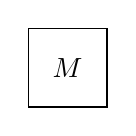
\begin{tikzpicture}[baseline=(current bounding box.center)]
    \draw (0,0) rectangle (1,1);
    \node at (0.5,0.5) {$M$};
  \end{tikzpicture}
  \approx
  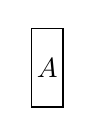
\begin{tikzpicture}[baseline=(current bounding box.center)]
    \draw (0,0) rectangle (0.4,1);
    \node at (0.2,0.5) {$A$};
  \end{tikzpicture}
  \cdot
  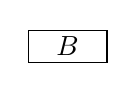
\begin{tikzpicture}[baseline=(current bounding box.center)]
    \draw (0,0) rectangle (1,0.4);
    \node at (0.5,0.2) {$B$};
  \end{tikzpicture}
\]

This problem can be translated into a numerical analysis problem of the following shape
\[
  \min_{A, B} \norm{M - AB}
\]

The matrices $A$ and $B$ can be obtained from eigenvectors of $M^TM$ and $MM^T$, but that's a huge, possibly dense matrix. So a more efficient way should be used, which also avoids the explicit formation of $M^TM$ and $MM^T$ because that would need a lot of memory.\\

\noindent Efficiently solving this problem requires:
\begin{itemize}
    \item low-complexity computation
    \item avoiding the explicit forming of $M^T M$ and $MM^T$
    \item exploiting the structure of $M$ (sparsity, similar columns, \ldots )
    \item ensuring that the solution is \emph{numerically stable}
\end{itemize}

\subsection{Support vector machines}

Let us consider the so-called ``decision problem'': given a set of values of many parameters (variables) ``label'' a person $i$ as ill or healthy, $y^i \in \{1, -1\}$.

The geometric intuition in two dimensions is given by \Cref{fig:19sett2}.
We would like to find the line that better splits the plane into two regions, because this could help to diagnose the next patient.
The rationale here is to maximize the space between the line and the nearest points (called \textbf{margin}), in order to have a better accuracy.\\

\noindent The distance between the two hyperplanes $(w_0, \vect{w}_+)$ and $(w'_0, \vect{w}_+)$ in \Cref{fig:19sett2} is computed as $\frac{2}{\norm{\vect{w}_+}}$,  so in order to maximize the distance between the planes we aim at minimizing $\norm{\vect{w}_+}$.
For each hyperplane that lies between $(w_0, \vect{w}_+)$ and $(w'_0, \vect{w}_+)$ the following holds
\[
	\begin{cases}
		\vect{w}_+ \vect{x}^i + w_0 \geq 1 \hspace{3cm} \text{if}\; \; y^i = 1\\
		\vect{w}_+ \vect{x}^i + w_0 \leq -1 \hspace{2.75cm} \text{if}\; \; y^i = -1
	\end{cases}
\]
    

\addtwopics{0.4}{pics/19sett/svm4.pdf}{0.4}{pics/19sett/svm5.pdf}{There are many possible boundaries that can be chosen as a model using many angular coefficients. Our best guess is the one that maximizes the distance between the line and the nearest points.}{fig:19sett2}

\noindent Under the hypotheses of this optimization problem, the maximum-margin separating hyperplane (assuming that any exists) is the solution of
\[
  \min\limits_{\vect{w}} \big\{\sqrnorm{\vect{w}_+}~:~y^i( \vect{w}_+ \vect{x^i} + w_0 ) \geq 1, ~ i = 1, \ldots, m \big\}
\]
       
In practice, most of the times there is no such line. 
To overcome this issue we introduce the concept of ``penalty'' that accounts for the number of points that are misclassified, through the following

\begin{definition}[SVM Primal problem]
We term Support Vector Machine primal problem (SVM-P) a convex constrained problem with complex constraints that is formalized as

\begin{equation}
\tag{SVM-P}
\begin{cases}
\min\limits_{\vect{w},\xi}{\sqrnorm{\vect{w}_+} + C \sum\limits_{i=1}^m \xi_i}\\
y^i( \vect{w}_+ \vect{x}^i + w_0 ) \geq 1 - \xi_i \, , \, \xi_i \geq 0 \, ,  \, \forall i = 1, \ldots, m 
\end{cases}    
\end{equation}

Where $C$ is an \textbf{hyper-parameter} that weights the violation of the separating margin.
\end{definition}


This definition formalizes the intuition that the approximated function may have a greater norm and lead to a very small misclassification error, or it could be the other way round.
  Both these solutions are acceptable and their performances depend only on the problem.

Whenever we are able to solve a multi-objective optimization problem we are also able to solve what is called the \textbf{dual problem}, which in our case has the following shape.

\begin{definition}[SVM Dual problem]
	We call Support Vector Machine dual problem (SVM-D) a convex constrained quadratic problem defined as 
\begin{equation}
\tag{SVM-D}
\begin{cases}
	\max\limits_{\alpha} \sum\limits_{i=1}^m \alpha_i - \frac{1}{2} \sum\limits_{i=1}^m \sum_{j=1}^m \alpha_i \ps{\vect{x^i}}{\vect{x^j}} \alpha_j\\
	\sum\limits_{i=1}^m y^i \alpha_i = 0\\
	0 \leq \alpha_i \leq C \, , \,  \forall i = 1, \ldots, m
\end{cases}    
\end{equation}
\end{definition}

\noindent The idea behind the theory of duality is to obtain the solution of a problem by solving an (apparently) different one.

\begin{lemma}
Given an optimal solution $\alpha^*$ for  the dual problem (SVM-D), then $\vect{w^*}_+ = \sum_{i=1}^{m} \alpha_i^* y^i \vect{x^i}$ is optimal for the primal problem (SVM-P).
\end{lemma}

A reader who has a deeper background in the field of machine learning knows that the scalar product in the dual form allows the usage of the so-called ``kernel trick''.
This mathematical transformation allows the mapping of the input space into a larger feature space where the points are more likely to be linearly separable.

Theoretically, the feature space can be infinite-dimensional, provided that the scalar product can be (efficiently) computed.

This whole course has the aim of presenting some techniques for solving efficiently \textbf{convex quadratic problems}, as the ones presented above.
